\chapter{Deployment Results and Verification}\label{chap:results}

In this chapter, we present the system as it is actually configured to deploy, based on
the committed Terraform configuration, Kubernetes manifests, Helm chart, and CI/CD
workflows in the \texttt{Ejada-A} repositories, rather than as designed on paper.

\section{The Five Services, as Deployed}\label{sec:primary-finding-one}
Figure~\ref{fig:topology} is the team's own architecture diagram for the deployed
system: the full path from a developer or shopper, through the public subnets, into the
private worker nodes and pods, and out to OCIR for image pulls.

\begin{figure}[p]
\centering
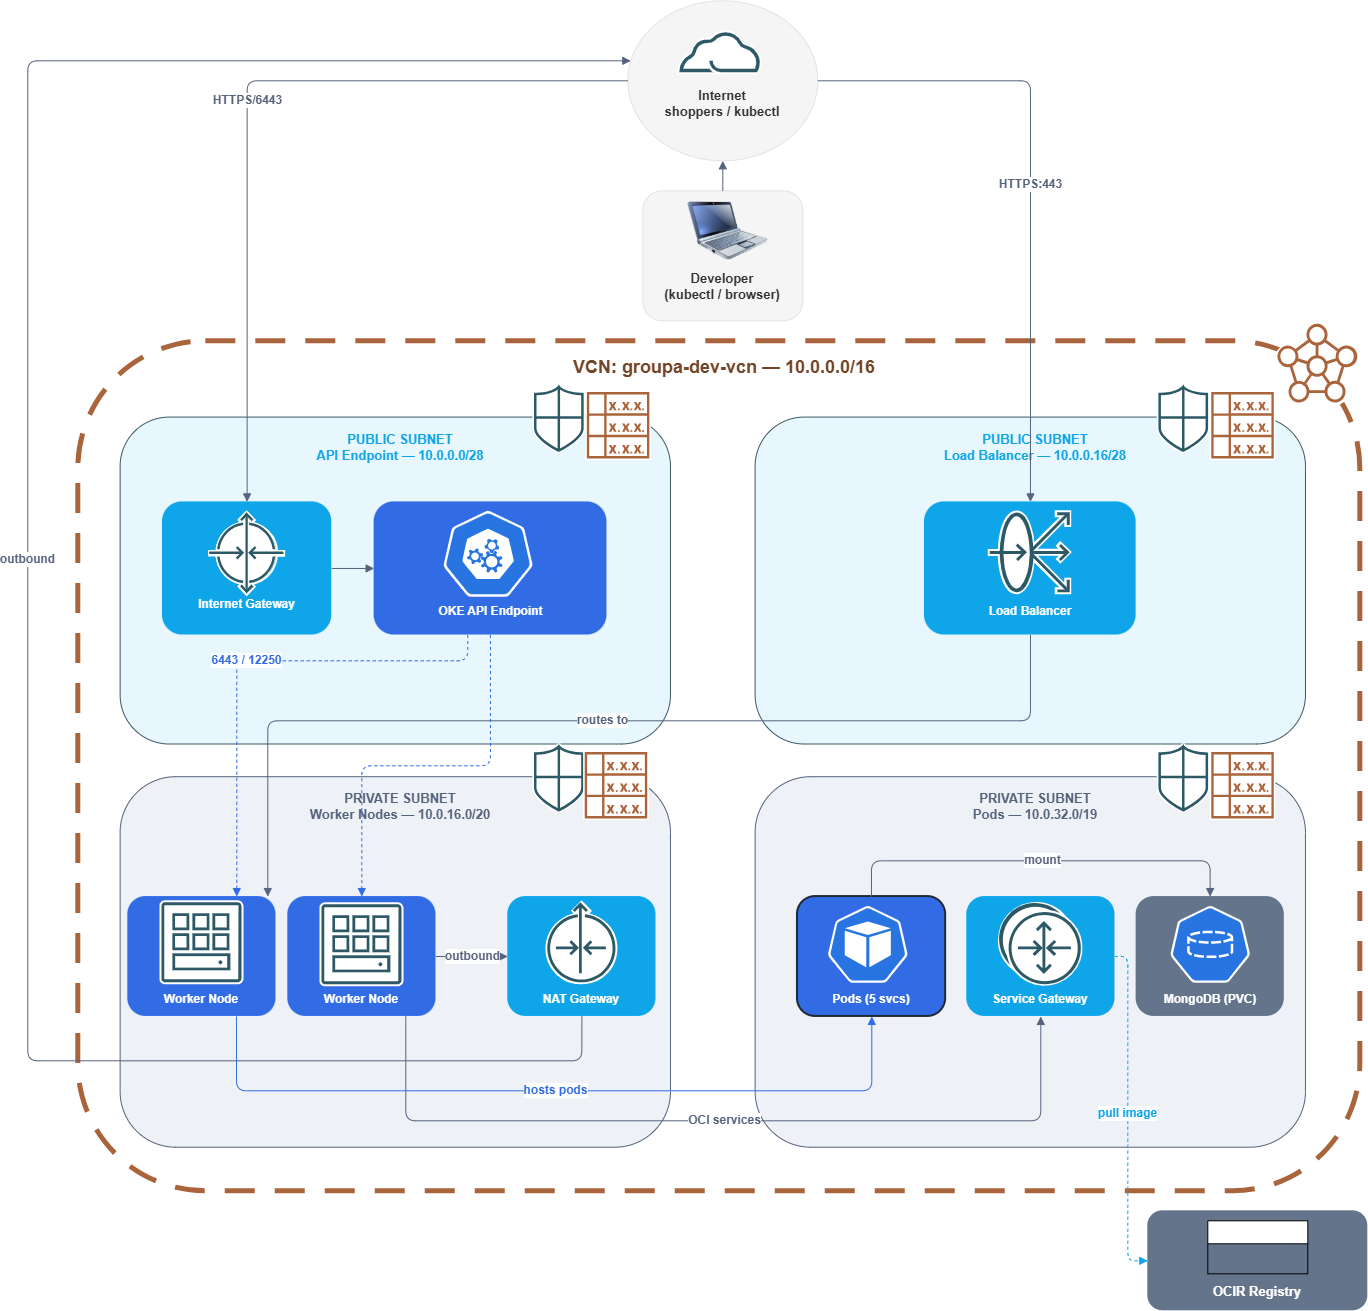
\includegraphics[width=\textwidth]{Figures/week4Architecture.png}
\caption{Deployed architecture inside VCN \texttt{groupa-dev-vcn} (\texttt{10.0.0.0/16}).
A developer reaches the OKE API endpoint over \texttt{HTTPS/6443} through the Internet
Gateway; shoppers reach the Load Balancer over \texttt{HTTPS:443}. Both public subnets
route into the private Worker Nodes subnet (\texttt{10.0.16.0/20}, two nodes, egress via
NAT Gateway) and Pods subnet (\texttt{10.0.32.0/19}, five services plus the shared
MongoDB PVC), which reaches OCI services, including pulling images from the OCIR
Registry, through the Service Gateway rather than the NAT path.}
\label{fig:topology}
\end{figure}

Figure~\ref{fig:app-access} narrows in on the application layer inside the Pods subnet:
the Ingress Controller's path-based routing to each of the five workloads, and the
shared MongoDB instance every one of them, including the frontend itself, connects to
directly.

\begin{figure}[H]
\centering
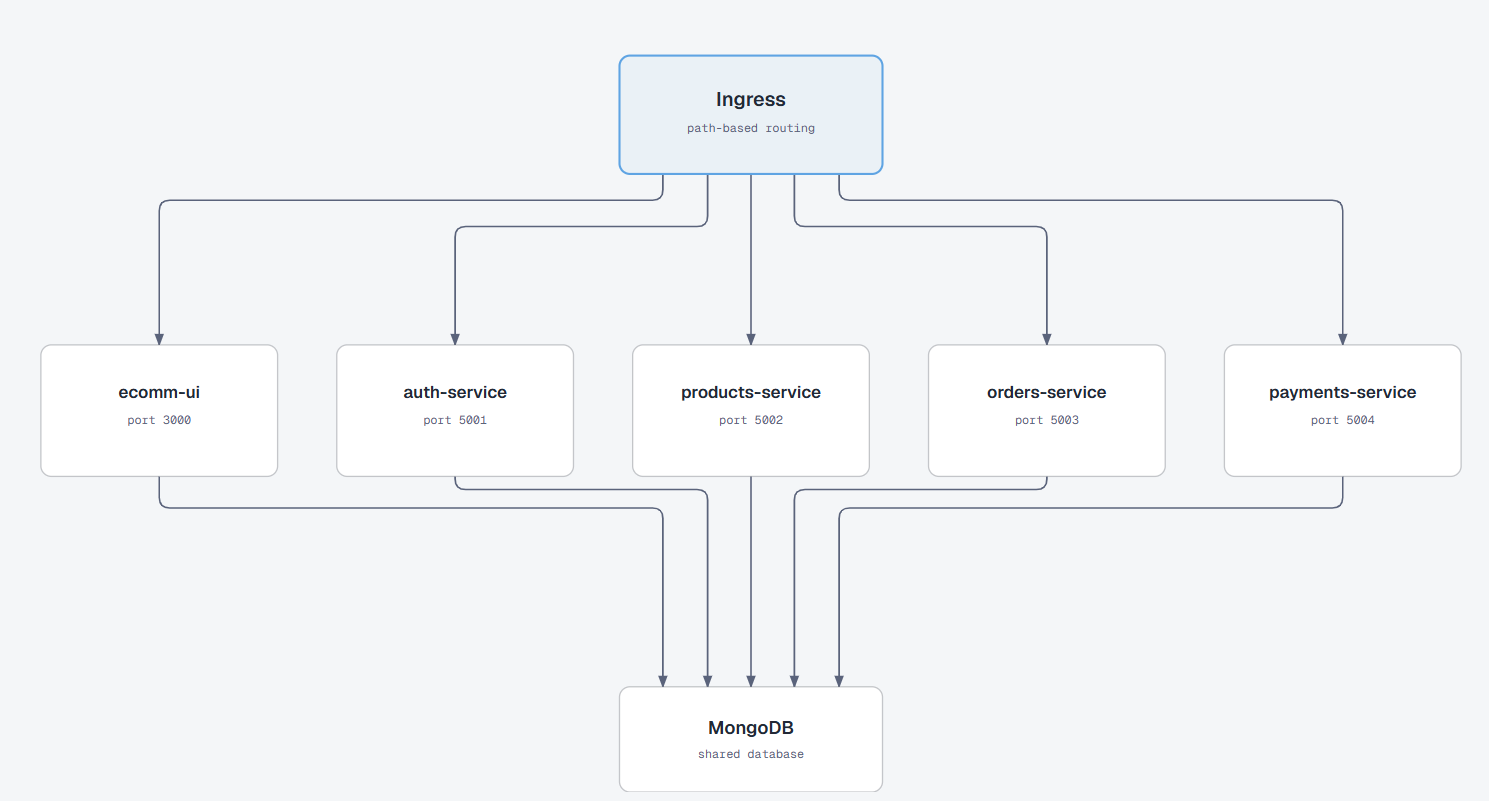
\includegraphics[width=0.92\textwidth]{Figures/appAccessStructure.png}
\caption{Application-layer access structure. The Ingress routes by path to
\texttt{ecomm-ui} and each of the four backend services by their internal ClusterIP
service name and port; every workload, including \texttt{ecomm-ui} itself, holds its own
connection to the single shared MongoDB instance.}
\label{fig:app-access}
\end{figure}

This corrects a simplification worth flagging: \texttt{ecomm-ui} is not a pure
stateless proxy in front of the four backend services. Most of its API routes do proxy
to the corresponding backend service, but it also holds its own direct MongoDB
connection (\texttt{src/lib/db.ts}) alongside that proxying.

Each backend service builds and pushes to its own OCIR repository under
\texttt{jed.ocir.io/axkjllkftxfz/shared-group-a-cmp/}, matching the domain boundaries set
out in Table~\ref{tab:domain-ownership}: \texttt{auth-service}, \texttt{products-service},
\texttt{orders-service}, \texttt{payments-service}, and \texttt{ecomm-ui}. The
one-repository-per-service pattern matches the registry design in
Section~\ref{sec:app-layer-design}, though the repository names themselves moved from
the design phase's \texttt{groupa-*-app} convention to the plural, per-service names
above.

\section{Traffic Routing and Autoscaling}\label{sec:primary-finding-two}
The ingress resource performs path-based routing from the single public host to each
backend service, as set out in Table~\ref{tab:ingress-routing}; compare this against the
routing designed during the assessment phase in Table~\ref{tab:routing-design}.

\begin{table}[H]
\centering
\caption{Path-based routing rules deployed in the ingress resource.}
\label{tab:ingress-routing}
\small
\begin{tabular}{lll}
\toprule
\textbf{Path} & \textbf{Routed to} & \textbf{Port} \\
\midrule
\texttt{/} & \texttt{ecomm-ui} & 80 \\
\texttt{/api/auth} & \texttt{auth-service} & 5001 \\
\texttt{/api/products} & \texttt{products-service} & 5002 \\
\texttt{/api/orders} & \texttt{orders-service} & 5003 \\
\texttt{/api/payments} & \texttt{payments-service} & 5004 \\
\bottomrule
\end{tabular}
\end{table}

Every workload, including the frontend, scales independently through its own
Horizontal Pod Autoscaler, deployed with a uniform policy across all five: a minimum of
2 replicas and a maximum of 5, scaling on 75\% CPU utilization (the raw Kubernetes
manifests additionally target 80\% memory utilization). This keeps every service at a
minimum of two replicas for redundancy while capping the maximum to bound cost, in place
of the per-service minimum and maximum designed during the assessment phase
(Table~\ref{tab:hpa-design}).

Table~\ref{tab:resource-sizing} lists the CPU and memory each pod requests and is capped
at; the four backend services all use the identical values, while the frontend and the
shared MongoDB instance are sized larger.

\begin{table}[H]
\centering
\caption{Per-pod resource requests and limits.}
\label{tab:resource-sizing}
\small
\begin{tabularx}{\textwidth}{>{\raggedright\arraybackslash}p{4.4cm} X X}
\toprule
\textbf{Workload} & \textbf{CPU request / limit} & \textbf{Memory request / limit} \\
\midrule
\texttt{auth-service}, \texttt{products-service}, \texttt{orders-service}, \texttt{payments-service} & 100m / 500m & 128Mi / 256Mi \\
\texttt{ecomm-ui} & 200m / 1000m & 256Mi / 512Mi \\
\texttt{mongodb} & 200m / 1000m & 512Mi / 1Gi \\
\bottomrule
\end{tabularx}
\end{table}

These per-pod values are a separate sizing decision from the node pool's own compute
shape in Section~\ref{sec:assumptions-limitations}: the node pool sizing bounds how much
total CPU and memory each worker node has to offer, while these requests and limits
bound how much of that capacity any single pod can claim. The HPA scales replica
\emph{count} against these per-pod requests, not against the node pool directly.

\section{The GitOps Deployment Pipeline}\label{sec:primary-finding-three}
The \texttt{argocd/ecommerce-app.yaml} Application resource, once applied, points ArgoCD
at the \texttt{helm/ecommerce-app} path of the \texttt{Terraform-code} repository:

\begin{lstlisting}[caption={\texttt{Terraform-code/argocd/ecommerce-app.yaml}}]
spec:
  source:
    repoURL: 'https://github.com/Ejada-A/Terraform-code.git'
    path: helm/ecommerce-app
  destination:
    namespace: ecommerce-ns
  syncPolicy:
    automated:
      prune: true
      selfHeal: true
\end{lstlisting}

With \texttt{selfHeal} enabled, a manual \texttt{kubectl edit} against a live Deployment
would be reverted on the next reconciliation; the Helm chart in Git is the only path
ArgoCD treats as authoritative, matching the source-of-truth split described in
Section~\ref{sec:data-evidence-weighting}.

\section{Verification Performed}\label{sec:quant-comparative-scenario}
This documentation was compiled from the repositories under the \texttt{Ejada-A} GitHub
organization rather than from a live session against the running cluster. What we
verified directly:

\begin{itemize}[leftmargin=1.4em]
  \item every ingress path, port, and HPA threshold in
        Section~\ref{sec:primary-finding-two} was read directly from the committed
        Kubernetes manifests and the Helm chart's templates and \texttt{values.yaml};
  \item the image-promotion pipeline in Section~\ref{sec:evaluation-criteria} was traced
        through each service's own \texttt{ci.yml} and the shared
        \texttt{update-helm.yml} workflow; and
  \item the domain-to-service mapping in Table~\ref{tab:domain-ownership} was confirmed
        against each service's own \texttt{server.ts} and data models.
\end{itemize}

We have not independently confirmed these against a live \texttt{kubectl get pods} or a
request against the public load balancer at the time of writing this documentation.

\section{Open Implementation Decisions}\label{sec:risk-analysis}
Two decisions were explicitly left open during the assessment phase and resolved with a
concrete default during the Terraform and Kubernetes build:

\begin{itemize}[leftmargin=1.4em]
  \item the OKE node pool's compute shape and OCPU/memory split, defaulted to
        \texttt{VM.Standard.A1.Flex} at 2 OCPUs and 16\,GB; and
  \item the database engine per service, resolved as one shared MongoDB instance for all
        five services rather than a separate database per service.
\end{itemize}

\section{Key Unknowns}\label{sec:key-unknowns}
This build does not cover multi-region or multi-availability-domain high availability,
an HTTPS listener on the ingress, or load testing against the deployed autoscaling
thresholds; all three are out of scope for this documentation rather than open failures.
